\documentclass{article}
\usepackage{amsmath}
\usepackage{amsfonts}
\usepackage{graphicx}
\usepackage{float}
\usepackage{subcaption}
\usepackage{bm}
\graphicspath{{./}}
\usepackage[left=1cm,right=1cm,top=1cm,bottom=1cm]{geometry}
\begin{document}
\title{Rotation Invariance using Second-order Convolutional Neural Networks}

\section{Introduction}
We propose a non-trivial filter filter for a Convolutional Neural Network (CNN) that is invariant to rotations of the input image around the center of the filter. 
In particular we show how to construct such non-trivial rotationally-invariant filter by using two convolutional neural network layers with a nonlinear ReLu after each convolution.
Our layer has the following two important properties that cannot both be attained by multiplication by a single filter.
One, it is rotationally invariant, and two, it is non-trivial. 
What we mean by non-trivial is that our single filter is able to distinguigsh a dumbbell from a donut, even if the donut looks exactly like the surface generated by a rotated dumbbell.
No actiong by a single linear filter can have both those properties since linearity implies the second property cannot hold given the first.
Furthermore, the filter does not need to be trained on rotated views of its input image.
In \cite{chengzhouhan}, Cheng et al. build a neural network that is essentially rotation invariant.
In \cite{jaderberg}, Jaderberg builds a neural network that is invariant to rotations (more generally, to affine transformations of the input).
However, both of those papers require that the network be trained on several transformed input representations in order for the network to learn to be rotationally invariant.
Relatedly, neither of those networks is guaranteed mathematically to be invariant to rotations of the input image (even for square images rotated a quarter turn, for example).
We construct a non-trivial rotationally invariant CNN architecture that does not need to be trained on multiple rotated views on an object.
Our filter is exactly rotationally invariant for rotations by a quarter turn, and the only reason it is only approximately invariant for other rotations is because of the rectangular nature of image pixels, which we compensate for by using gaussian blurring.
For sufficiently high-resolution pixels (or for pixels arranged finely enough along grid lines in polar coordinates) our method is guaranteed to be rotationally invariant to arbitrary precision.
Na\"ively, one might expect that rotationally invariant filters satisfy our goal.
However, as pointed out above, since a single filter is linear in its inputs, any rotationally invariant filter will return the same value for an image and for any weighted average of various rotations of that image.
We find this problematic because we would like our rotationally invariant filter to be able to distinguish objects like a donut from a dumbbell, even though if you rotate a dumbbell you get an object that looks like a donut.
We show that two layers of rotationally invariant second-order filters have the desired properties.

\section{Related Work}
In \cite{marcos}, they generate exact rotation invariance over a finite number of rotations by taking the maxpool over a set of rotated filters.

\section{Defining a rotationally invariant filter}
No standard first-order filter is able to accomplish that task because first-order filters are linear in their inputs, so if they are invariant to rotation then they are also necessarily equally triggered by an image of that object and by a weighted average of images of rotations of that object.

We construct an (approximately) rotationally-symmetric filter as follows. 
We assume a square filter of side length $2h + 1$. 
The pixels are defined by $\mathbf x = (x,y),\text{ for } x,y\in [-h,h]$ we define the radius $r$ of a pixel as $r_{\mathbf{x}} = ||x||_2$. 
We can therefore construct an approximately rotationally-invariant basis filter by setting the filter value $f_n(\mathbf{x})$ to be equal to
$f(\mathbf{x}) = P(n,\sigma,r_x)$ 
where $n$ is the radius parameter for the desired filter, $\sigma$ is the standard deviation of the blurring gaussian for the filter, and $P(n, \sigma, r_x)$ is the gaussian probability density value of the point $r_x$ for the gaussian centered at $n$ with standard deviation $\sigma$.

\begin{figure}[h]
\centering
\begin{subfigure}[t]{.3\textwidth}
 \centering
 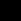
\includegraphics[width=1in]{basis}
 \caption{Our rotationally symmetric basis filter of radius 5 pixels}
\end{subfigure}
\begin{subfigure}[t]{.3\textwidth}
 \centering
 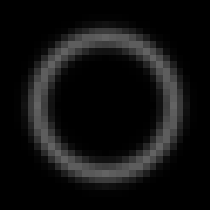
\includegraphics[width=1in]{rotbasis45}
 \caption{That basis filter rotated by 45 degrees counterclockwise (using bilinear interpolation to fit rotated pixels)}
\end{subfigure}
\begin{subfigure}[t]{.3\textwidth}
 \centering
 
\includegraphics[width=1in]{diffbasisrot45}
 \caption{The difference in pixel intensity between the basis filter and the rotated basis filter (hardly discernable)}
\end{subfigure}
\end{figure}

\bibliography{traversr}{}
\bibliographystyle{plain}
\end{document}
